\name{fig}{plot a graph}{plotting graphs}

\begin{synopsis}
 \item[fig] [ --F $F$ ] [ --R $R$ ] [ --W $W$ ] [ --H $H$] [ --o $xo$ $yo$ ]
	    [ --g $G$ ]  [ --p $P$ ] 
 \item[\ ~~~] [ --s $S$ ] [ --f $file$ ] [ --t ] [ {\em infile} ]
\end{synopsis}

\begin{qsection}{DESCRIPTION}
This command draws a graph using information from the input file
{\em infile}. 
If {\em infile} is not assigned, data is read from the standard input.
This command is similar to the unix command ``graph'' but includes
some labeling functions.
The output file comes with a sequence of commands for direct printing.
For this reason, in case the output is printed on the screen,
one should use the ``xgr'' command.
In case the output is printed in postscript, one should use the
``psgr'' command.
\end{qsection}

\begin{options}
	\argm{F}{F}{factor}{1}
	\argm{R}{R}{rotation angle}{0}
	\argm{W}{W}{width of figure($\times 100$mm)}{1}
	\argm{H}{H}{height of figure($\times 100$mm)}{1}
	\argm{o}{xo \; yo}{origin in mm}{20 20}
	\argm{g}{G}{draw grid($0 \sim 2$)\\
			\begin{tabular}{cccc}
			&\includegraphics[width=2cm]{fig/g0.eps}
			&\includegraphics[width=2cm]{fig/g1.eps}
			&\includegraphics[width=2cm]{fig/g2.eps}\\
			$G$&0&1&2	 
			\end{tabular}\\\hspace*{\fill}}{2}
	\argm{p}{P}{pen number($1 \sim 10$)}{1}
	\argm{s}{S}{font size($1 \sim 4$)}{1}
	\argm{f}{file}{The file assigned after this option is read
                       before {\em infile}, that is, this option gives
                       preference.}{NULL}
	\argm{t}{}{transpose $x$ and $y$ axes}{FALSE}
\end{options}

\begin{qsection}{EXAMPLE}
Data in {\em data.fig} file is plotted in an X terminal in the
example below:
\vspace{-3mm}
\begin{quote}
 \verb!fig data.fig |xgr!
\end{quote}
\vspace{-3mm}
In this example, data in {\em data.fig} file is written in postscript,
and seen with ghostview:
\vspace{-3mm}
\begin{quote}
 \verb!fig data.fig | psgr | ghostview -!
\end{quote}
\vspace{-3mm}
\end{qsection}

\vspace{-1cm}
\begin{qsection}{USAGE}
��\vspace{-1cm}
\end{qsection}

\begin{qsection}{\ ~~~COMMAND}
The input data file can contain commands and data.
Commands can be used for labeling, scaling, etc.
Data is written in the ($x ~y$) coordinate pair form.
Command values can be overwritten by entering new command values.
\end{qsection}

\vspace{-1cm}
\begin{qsection}{\ ~~~COMMAND LINES}
\begin{minipage}[t]{5.5cm}
x [mel $\alpha$]~ $xmin$ ~$xmax$ [$xa$]\\
y [mel $\alpha$]~ $ymin$ ~$ymax$ [$ya$]\\
\end{minipage}
\begin{minipage}[t]{9cm}
Assigns $x$ and $y$ scalings.
Marks can be assigned in $x$ and $y$ axes through $xa$ and $ya$.
If no assigned of $xa$ and $ya$ is done,
then $xa = xmin$ and $ya = ymin$.
If the optional ``mel $\alpha$'', where $\alpha$ must be
a number (for example, mel 0.35), is used,
then labeling is undertaken as a frequency transformation of
a minimum phase first order all-pass filter.
\end{minipage} \\

\begin{minipage}[t]{5.5cm}
xscale ~$x_1$ $x_2$ $x_3$ $\cdots$\\
yscale ~$y_1$ $y_2$ $y_3$ $\cdots$
\end{minipage}
\begin{minipage}[t]{9cm}
Assigns the points $x_1, x_2,x_3,\cdots$
and $y_1,y_2,y_3,\cdots$ in $x$ and $y$ axes.
These points can be assigned with numbers or marks,
Also, when a mixture of not-a-number $+$ number (for example, '2,*3.14)
is needed, the following function should be used:

\begin{tabular}{cl}
s & draws marks with half size.\\
$\backslash$& only writes number.\\
@ & does not write anything \\
  & but assigns positions of marks.\\
none of the above & only marks are written.
\end{tabular}\\

Whenever the character is inside quotes,
it appears in the position assigned
by the string that precedes it.
Please refer to the commands ``x/yname'' for information on
special characters.\\
(Example)\\
x ~0 ~5\\
xscale 0~1.0 ~s1.5 ~'2 ~$\backslash$2.5 ~'3.14 ~''$\backslash$pi'' ~@4 ~''x'' ~5\\

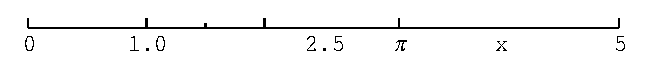
\includegraphics[width=9cm]{fig/scale.eps}
\end{minipage}\\

\begin{minipage}[t]{5.5cm}
xname ~''$text$''\\
yname ~''$text$''\\
\end{minipage}
\begin{minipage}[t]{9cm}
Labels $x$ and $y$ axes.
$text$ should be inside quote.
Inside $text$, \TeX commands can be used.
Also, characters such as those that can be obtained
with \TeX can be written with this command.
\end{minipage}\\

\begin{minipage}[t]{5.5cm}
 print ~x ~y ~''$text$'' [$th$]\\
 printc ~x ~y ~''$text$'' [$th$]
\end{minipage}
\begin{minipage}[t]{9cm}
This command writes $text$ in the assigned position (x ~y).
The option $th$ assigned the rotation degree.

\begin{tabular}{cc}
\includegraphics{fig/fig-print1.eps}&  
\includegraphics{fig/fig-print2.eps}\\
print&printc
\end{tabular}p
\end{minipage}\\

\begin{minipage}[t]{5.5cm}
title ~x ~y ~''$text$'' [$th$]\\
titlec ~x ~y ~''$text$'' [$th$]
\end{minipage}
\begin{minipage}[t]{9cm}
This command is same as print(c).
However, the basic unit is expressed in absolute value mm.
The reference point is on the botton-left.
\end{minipage}\\

\begin{minipage}[t]{5.5cm}
csize ~h [w]
\end{minipage}
\begin{minipage}[t]{9cm}
This command assigns in mm the character width and height,
to be used in the following commands:\\
x/yscale��x/yname��print/c��title/c\\
When the value of $w$ is omitted, $w$ is made equal to $h$.
The default values for the option --{\bf s} follows:
\begin{tabular}{ccc}

--{\bf s} &w &h  \\ \hline
1 &2.5 &2.2\\
2&5&2.6\\
3&2.5&4.4\\
4&5&4.4
\end{tabular}\\

\end{minipage}\\

\begin{minipage}[t]{5.5cm}
 pen ~$penno$
\end{minipage}
\begin{minipage}[t]{9cm}
This command chooses the variable $penno$.
$1 \leq  penno \leq 10$.????????????????????????????????????????????
Please refer to appendix.
\end{minipage}\\

\begin{minipage}[t]{5.5cm}
line ~$ltype$ [$lpt$]
\end{minipage}
\begin{minipage}[t]{9cm}
This command assigns the type $ltype$ of the line which will connect
data as well as the $lpt$ pace. $lpt$ is on mm unit.
When $ltype$=0: no line is used to connect coordinate points.
1:~solid~~2:~dotted~~3:~dot and dash~~4:~broken~~5:~dash
Please refer to the appendix.\\
	
\end{minipage}\\

\begin{minipage}[t]{5.5cm}
xgrid ~$x_1$ ~$x_2$ ~$\cdots$\\
ygrid ~$y_1$ ~$y_2$ ~$\cdots$
\end{minipage}
\begin{minipage}[t]{9cm}
This command makes grids in the positions $x_1$ $x_2$ $\cdots$,
$y_1$ $y_2$ $\cdots$.\\
(Example)\\
\begin{minipage}[t]{4.3cm}
 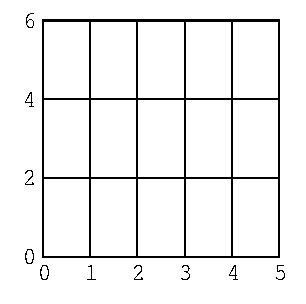
\includegraphics[width=4cm]{fig/grid.eps}
\end{minipage}
\begin{minipage}[b]{4.5cm}
\baselineskip 5pt
x 0 5\\
y 0 6\\
xscale 0 1 2 3 4 5\\
yscale 0 2 4 6

\vspace{3mm}
xgrid 1 2 3 4\\
ygrid 2 4
\vspace*{1cm}
\end{minipage}
\end{minipage}\\


\begin{minipage}[t]{5.5cm}
mark ~$label$ [$th$]
\end{minipage}
\begin{minipage}[t]{9cm}
This command draws a mark in the assigned coordinate position.
The option $th$ assigns angle(degree) that the string will be draw.
If $label$ is assigned $\backslash 0$, the mark is released.
The way to write marks and special characters can be seen
at the $label$ section of data explanation.
\end{minipage}\\

\begin{minipage}[t]{5.5cm}
hight ~$h$ [$w$]\\
italic ~$th$
\end{minipage}
\begin{minipage}[t]{9cm}
This command defines the size of the label through its
height $h$(mm) and width $w$(mm) whenever it is assigned
and allows for writing a label in italic.
\end{minipage}\\

\begin{minipage}[t]{5.5cm}
circle ~x ~y ~$r_1$ ~$r_2$ ~$\cdots$\\
xcircle ~x ~y ~$r_1$ ~$r_2$ ~$\cdots$\\
ycircle ~x ~y ~$r_1$ ~$r_2$ ~$\cdots$

\end{minipage}
\begin{minipage}[t]{9cm}
This command writes a circle with radius $r_1$ ~$r_2$ ~$\cdots$
with center on the coordinate ($x$,~$y$).
Also, the unit for the radius $r_x$ in the circle command is mm,
for the xcircle command is the scale of the $x$ axis and
for the ycircle command is the scale of the $y$ axis,
as can be seen in the figure below.\\
(Example)\\
\begin{minipage}[t]{4.3cm}
 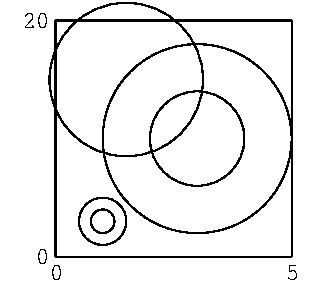
\includegraphics[width=4cm]{fig/circle.eps}
\end{minipage}
\begin{minipage}[b]{4.5cm}
\baselineskip 5pt
x 0 5\\
y 0 20\\
xscale 0 5\\
yscale 0 20

\vspace*{3mm}
xcircle 3 10 1 2\\
ycircle 1 3 1 2\\
circle  1.5 15 13\\
\vspace*{7mm}
\end{minipage}
\end{minipage}\\

\begin{minipage}[t]{5.5cm}
box ~$x_0$ $y_0$ $x_1$ ~$y_1$ [~$x_2$ $y_2$ $\cdots$ ]\\
paint ~$type$
\end{minipage}
\begin{minipage}[t]{9cm}
This command draws a rectangle with paint $type$
connecting ($x_0$ $y_0$) and ($x_1$ $y_1$) through a solid line.
The line which connects ($x_0$ $y_0$) and ($x_1$ $y_1$) forms
a diagonal of the rectangle.
Also, if $x_2$ $y_2$ $\cdots$ are assigned, a polygon is draw connecting
($x_0$ $y_0$),($x_1$ $y_1$),($x_2$ $y_2$),$\cdots$.
In this case, Please do not use paint $type$ different from 1.
The default of paint is 1.\\

(Example)\\
\begin{minipage}[t]{4.3cm}
 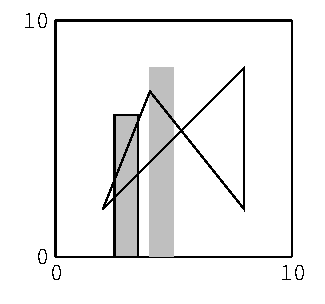
\includegraphics[width=4cm]{fig/box.eps}
\end{minipage}
\begin{minipage}[b]{4.5cm}
\baselineskip 5pt
x 0 10\\
y 0 10\\
xscale 0 10\\
yscale 0 10

\vspace*{3mm}
paint 18\\
box 2.5 0 3.5 6\\
paint -18 \\
box 4 0 5 8\\
paint 1\\
box  2 2 8 8 8 2 4 7
\end{minipage}
\end{minipage}\\

\begin{minipage}[t]{5.5cm}
clip ~$x_0$ $y_0$ $x_1$ ~$y_1$ 
\end{minipage}
\begin{minipage}[t]{9cm}
This command allows for drawing only inside the box defined by
($x_0$ $y_0$), ($x_1$ $y_1$).
When the coordinates ($x_0$ $y_0$), ($x_1$ $y_1$) are omitted,
then the clip command is released.\\

(Example)\\
\begin{minipage}[t]{4.3cm}
 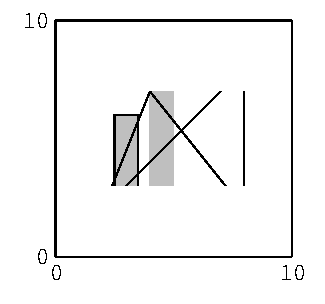
\includegraphics[width=4cm]{fig/clip.eps}
\end{minipage}
\begin{minipage}[b]{4.5cm}
\baselineskip 5pt
x 0 10\\
y 0 10\\
xscale 0 10\\
yscale 0 10

\vspace*{3mm}
clip 2 3 9 7\\
paint 18\\
box 2.5 0 3.5 6\\
paint -18 \\
box 4 0 5 8\\
paint 1\\
box  2 2 8 8 8 2 4 7
\end{minipage}
\end{minipage}\\

\begin{minipage}[t]{5.5cm}
\# any comment
\end{minipage}
\begin{minipage}[t]{9cm}
This is used for comment lines.
Whatever is written after this symbol
is ignored by the fig command.
\end{minipage}\\
\end{qsection}

\begin{qsection}{\ ~~~DATA LINES}
\begin{minipage}[t]{5.5cm}
 x ~y [$label$~ [$th$]]
\end{minipage}
\begin{minipage}[t]{9cm}
The coordinates (x ~y) are scaled by the values assigned in the
command lines.
If a string is written on $label$, then it will be written
in the (x ~y) position.
No empty character (eg., space character) should be left in $label$.
When $label$ is assigned in mark command,
$label$ replacement will take place only for this coordinate.
The option $th$ assigns the angle.\\
If $\backslash n$, where $0 \leq n \leq 15$, is assigned to $label$,
the corresponding mark is draw (refer to the appendix for the types of
marks).
When a minus sign is written before mark number,
then the connecting line between marks passes through the center of
each mark.\\
If a minus sign is not included, then connecting lines do not pass
through the center of each mark.
When $n=16(\backslash 16)$, a small circle is written with
diameter defined by the hight command.
Also, special character and ascii character can be written through
code number when $n>32$.
\end{minipage}\\

\begin{minipage}[t]{5.5cm}
 eod\\
EOD
\end{minipage}
\begin{minipage}[t]{9cm}
This is the end of data sign.
Coordinates before and after the eod sign are not connected.
\end{minipage}
\end{qsection}
\newpage
\begin{qsection}{APPENDIX}
{\large \hspace{-1.5ex}$\bullet$
The following type of marks can be defined through $label$:}

\begin{center}
\leavevmode
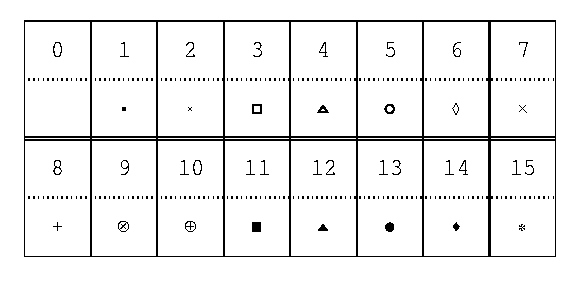
\includegraphics[width=12cm]{fig/mark.eps} \\
\end{center}


{\large \hspace{-1.5ex}$\bullet$
The following types of pen and line can be defined:}\\
\hspace{3mm}[When output is obtained through the command ``psgr'']

\leavevmode
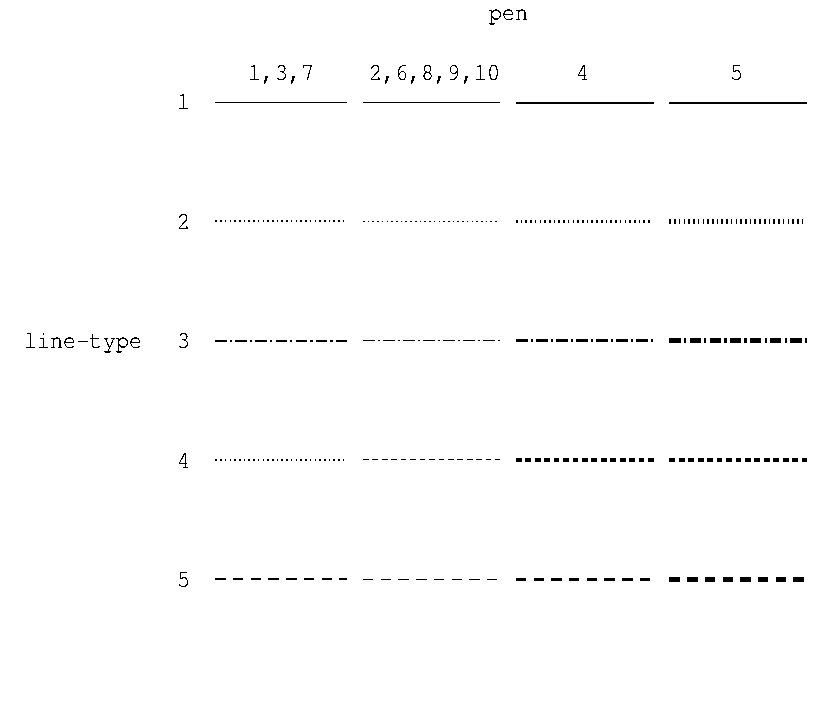
\includegraphics{fig/pen-line.eps} \\

(Attention)~~ The types of output generate through the pen command
depends on the printer(Please try printing this page).
\newpage
[When output is obtained through the command ``xgr'']\\
The following colors can be used.\\

\begin{center}
\begin{tabular}{|c|c|c|c|c|c|c|c|c|c|c|}
 \hline
 pen type& 1& 2& 3& 4& 5& 6& 7& 8& 9&10  \\ \hline
 color   & black& blue& red& green& pink& orange& emerald& gray&brown & 
 dark blue \\ \hline
\end{tabular}\\
\end{center}

\vspace{5mm}
{\large \hspace{-1.5ex}$\bullet$ paint type:}\\
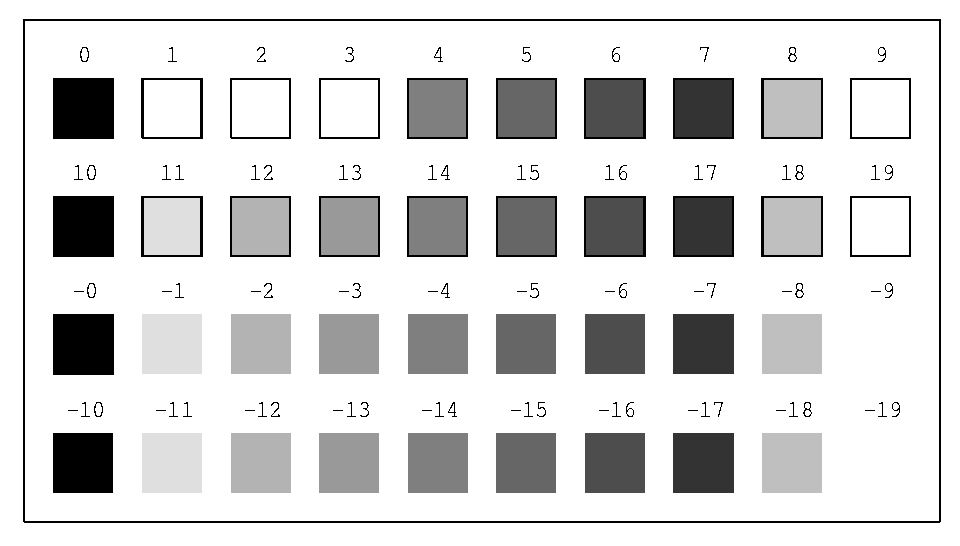
\includegraphics{fig/paint.eps}\\
(Attention)~~~From $1 \sim 3$ only a frame is draw,
and for $-9$ and $-19$ the center is white and no frame is draw.

\end{qsection}
